\section{Service Flexibility Agreement}
\label{sec:sfa}

In current PaaS architectures, the framework grants a certain flexibility to applications.
For example, an application can ask the PaaS framework to spawn more or less VMs or Linux containers\footnote{http://docs.cloudfoundry.org/concepts/architecture/warden.html} according to its needs.
However, the flexibility is entirely controlled by the application.
The intuition behind SFA is to delegate some of the flexibility control to the PaaS framework while still guaranteeing the end user satisfaction.
With respect to a traditional SLA, the SFA adds a few new dimensions: the possibility for the required resources to vary in time, plus the possibility to qualify violations of the required performance.

\begin{figure}[h]
\centering
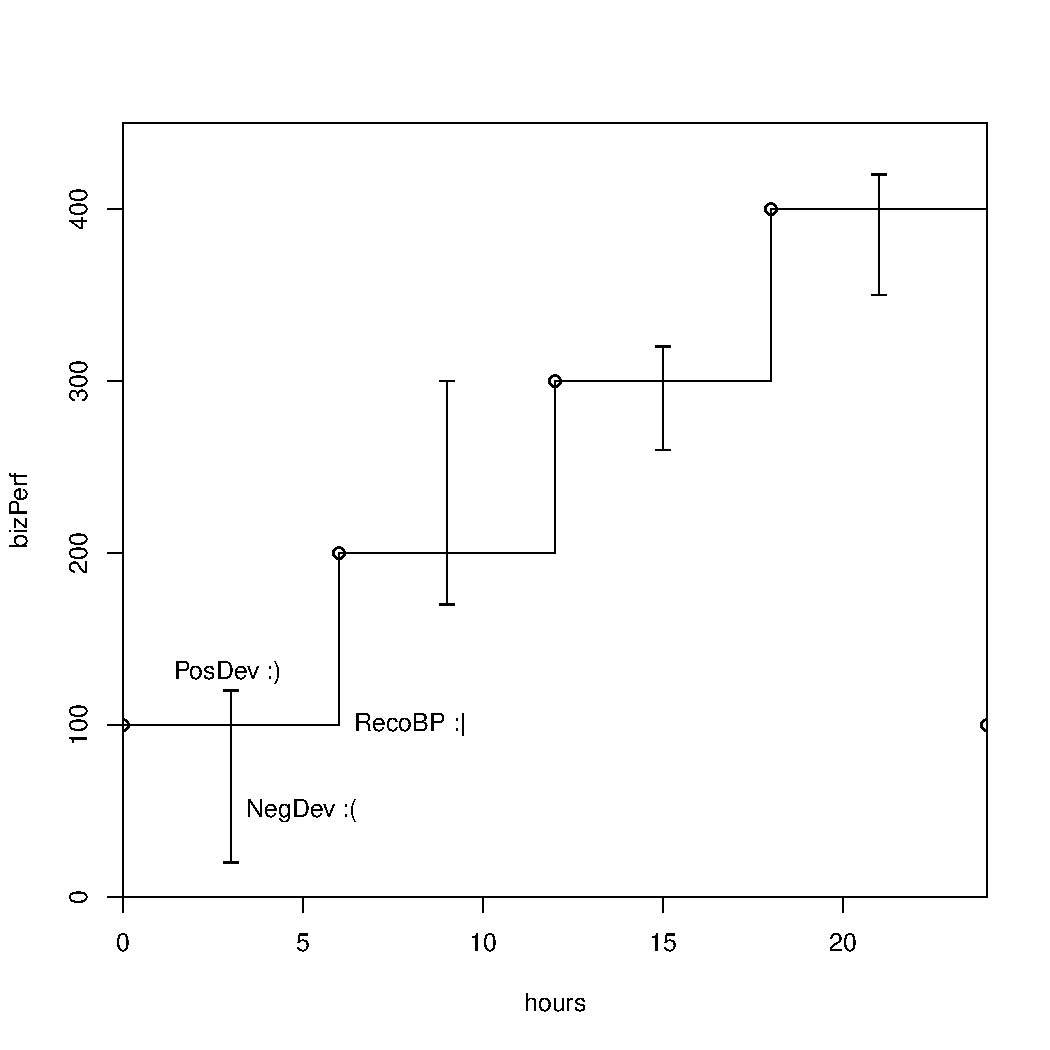
\includegraphics[width=0.99\linewidth]{generated/SFA-candles.pdf}
\caption{Service Flexibility Agreement representation}
\label{fig:SFA}
\end{figure}

\begin{listing}[ht]
\begin{minted} [frame=single, linenos]{yaml}
SFA:
  - Start: 00:00
    End: 06:00
    RecoBP: 100 Hz
    PosDev: 100 Hz/H
    NegDev: 50 Hz/H
  - Start: 07:00
    End: 12:00
    RecoBP: 300 Hz
    PosDev: 50 Hz/H
    NegDev: 200 Hz/H

WorkingModes:
  - WMName: WM1
    actuator: 'cf scale myApp -i 3'
    defaultPower: '300 W'
    maxBusinessPerf: '100 Hz'
  - WMName: WM2
    actuator: 'cf scale myApp -i 5'
    defaultPower: '500 W'
    maxBusinessPerf: '150 Hz'
\end{minted}
\caption{SFA example}
\label{lst:SFA}
\end{listing}

As shown in listing~\ref{lst:SFA} and also represented graphically in figure~\ref{fig:SFA}, for each time frame the SFA defines a recommended business performance (RecoBP). 
The business performance is one of the KPIs of the application.
It is expressed in Hertz: a number of items processed per unit of time.
For example, for a Web server it is the number of pages served per minutes, for a video transcoding service it will be how many videos can be transcoded per minutes.

We then define a concept called the "Happy points", noted "H".
This is an abstraction of the end-user satisfaction.
An application having zero Happy points means that the end user is reasonably satisfied.
An application being allocated exactly the number of resources corresponding to the RecoBP collects 0 Happy points.
This situation corresponds to the traditional SLA threshold.
The positive and negative deviations (PosDev and NegDev) declared in the SFA are then the way that each application "reacts" to being given more or less resources resources than the RecoBP.
Indeed, some applications such as video transcoding can benefit to receive temporarily more resources because they can process more videos and thus make their end user happier. 
This kind of application reacts linearly to the amount of resources it is allocated.
On the other hand, an application such as a web server typically have a "turning point" in their relation between performance and resources.
Indeed, giving them less that a certain level of resources (such as the number of front-end VMs) will start to augment the delay in delivering web pages, while giving more that a threshold will not have any perceptible impact on the end user.

We further define the Working Modes (WM) of an application.
A WM corresponds to a set of resources allocated by the PaaS to an application.
We associate to each WM a default power consumption and the maximum business performance it can offer.
In practice, a WM corresponds to a number of VMs or Linux Containers, each running instances of the application.
Using the SFA, it is now possible to compute the number of Happy points provided by each WM for each time slot.








\ms{We may refer to a function name like HappyPoints that as input receives performance, and as output gives the number of happy points}

%\ms{I believe more concrete definition is required. We need to establish a better relationship between working mode and SFA. We need better describe working mode and to remove green points.}

%\ms{Or we don't need to refer/define working mode. SFA already corresponds to working mode concept, that is SFA provides various performance levels with different power consumptions}

